%! Author = kubec
%! Date = 27.03.2024

% Preamble
\documentclass[11pt]{article}

% Packages
\usepackage{amsmath}
\usepackage{mathtools}
\usepackage{ragged2e}
\usepackage [utf8]{inputenc}
\usepackage{blindtext}
\usepackage{wrapfig}
\usepackage{xcolor}
\usepackage {polski}
\usepackage{multicol}
\usepackage[a4paper, total={5.7in, 8in}]{geometry}
\usepackage{graphicx}
\usepackage{amstex}
\usepackage{csvsimple}
\usepackage{changepage}
\usepackage{enumitem}
\usepackage[english]{babel}
\usepackage{biblatex}
\usepackage{caption}

\newenvironment{changemargin}[2]{%
    \begin{list}{}{%
        \setlength{\topsep}{0pt}%
        \setlength{\leftmargin}{#1}%
        \setlength{\rightmargin}{#2}%
        \setlength{\listparindent}{\parindent}%
        \setlength{\itemindent}{\parindent}%
        \setlength{\parsep}{\parskip}%
    }%
        \item[]}{\end{list}}

% Document
\begin{document}
    \begin{flushright}
        \large{
            Igor Czerwiec - 277680\\
            Filip Kubecki - 272655
        }\\
    \end{flushright}
    \begin{center}
        \large{Fizyka 3.1}\\
        \vspace{2mm}
        \LARGE{\textbf{Skalowanie termopary i wyznaczanie temperatury krzepnięcia wody}}\\
        \vspace{3mm}
        \huge{Nr ćwiczenia: 20a}\\
        \vspace{1cm}
    \end{center}
    \begin{flushright}
        \large{
            Data wykonania ćwiczenia: 21.03.2024r\\
            Data oddania sprawozdania: 03.04.2024r
        }\\
    \end{flushright}

    \section{Wstęp}
    Celem ćwiczenia jest wyznacznie współczynnika termoelektrycznego termopary oraz wyznaczenie temperatury krzepnięcia wody.\\
    \textbf{Wykorzystane przyrządy pomiarowe:}
    \begin{itemize}
        \itemsep0em
        \item Multimetr Sanwa PC7000
        \item Termometr (błąd pomiarowy $\pm$0.1 $^\circ$C)
        \item Stoper (błąd pomiarowy 0.01 s)
        \item Termopara
    \end{itemize}
    \subsection*{Przebieg doświadczenia}
    \textbf{1. Skalowanie termopary}\\
    \indent Do stalowego garnka nalewamy wody tak, aby
    linia wody znajdowała się około 3 cm poniżej
    krawędzi garnka. Termos zasypujemy lodem i
    dolewamy zimnej wody, aby uzupełnić luki i
    zwiększyć powierzchnię styku ośrodka z
    termoparą. Do garnka oraz termosu wkładamy
    przez odpowiednie otwory końce termopary.
    Do garnka wkładamy również termometr
    wzorcowy. Termoparę podłączamy zgodnie z
    rysunkiem do multimetru ustawionego na
    pomiar napięcia. Następnie włączamy kuchenkę
    i podgrzewamy wodę w garnku. Notujemy
    temperaturę w garnku oraz napięcie na
    termoparze. Pomiary powinny odbywać się od
    temperatury pokojowej do około 60 ℃. Kolejne
    pomiary wykonujemy co 2 ℃.\\
    \newpage
    \noindent\textbf{2. Wyznaczanie temperatury krzepnięcia wody}\\
    \indent Napełnić termos mieszaniną wody z lodem. Naczynie termiczne napełnić w 1/3 zimną wodą, dodać
    dwie płaskie łyżki soli kuchennej i poczekać aż się rozpuści (zamieszać). Naczynie dopełnić do 3/4 lodem
    z zamrażarki. Nabrać do strzykawki ok. 5 ml ciepłej wody z kranu. Przelać wodę do szklanego naczynka
    pomiarowego. Naczynko zatkać korkiem. Spojenie termopary umieścić w naczynku z ciepłą wodą tak,
    by termopara była zanurzona w wodzie, ale nie dotykała naczynka. Delikatnie zamocować naczynko w
    statywie i zanurzyć w roztworze lodu z wodą i solą. Uruchomić stoper i w czasie procesu chłodzenia
    wody (ok. 25 minut) co 20 s notować czas i napięcie termoelektryczne.

    \subsection*{Zastosowana teoria}\\
    \indent Woda przechodząc z stanu ciekłego do stanu stałego w trakcie
    przemiany fazowej pozbywa się energii dzięki czemu można
    zaobserwować dokładny moment przemiany fazowej.
    Przedstawia się go jako wypłaszczenie na wykresie zależności
    napięcia termoelektrycznego od czasu przy ciągłym
    ochładzaniu. Środek takiego wypłaszczenia to napięcie
    odpowiadające temperaturze krzepnięcia a odległość od
    niego do punktu przegięcia wykresu możemy uznać jako
    niepewność tej wartości.\\

    \noindent\textbf{Termopara} - element obwodu elektrycznego składający
    się z dwóch różnych przewodników, wykorzystujący
    zjawisko Seebecka, zachodzące na ich styku. Termopara
    jest wykorzystywana jako czujnik temperatury, rzadziej
    jako źródło zasilania o bardzo niskim napięciu i relatywnie
    wysokim prądzie.\\

    \noindent\textbf{Zjawisko Seebecka} - zjawisko termoelektryczne polegające na powstawaniu siły elektromotorycznej w
    obwodzie zawierającym dwa metale lub półprzewodniki, gdy ich złącza znajdują się w różnych
    temperaturach. Odkryte w 1821 roku przez fizyka niemieckiego (pochodzenia estońskiego)
    Th. J. Seebecka. Zjawisko to jest wykorzystywane m.in. w termoparze.\\

    \indent Skalowanie termopary polega na wyznaczeniu siły termoelektrycznej powstającej na zaciskach
    termopary w sytuacji gdy jedno ze złączy znajduje się w temperaturze odniesienia(w tym przypadku
    0 ℃) a temperatura drugiego złącza zmienia się przy czym jego temperaturę badamy jednocześnie za
    pomocą termometrów. Dzięki tym danym jesteśmy w stanie sporządzić wykres zależności napięcia od
    temperatury. Będzie to zależność liniowa której współczynnik kierunkowy będzie równy
    współczynnikowi termoelektrycznemu termopary.\\
    \newpage
    \indent Dzięki współczynnikowi termoelektrycznemu możemy obliczyć dokładną temperaturę termopary na
    podstawie napięcia między jej zaciskami zgodnie z wzorem poniżej:
    \begin{gather*}
        U=\alpha\cdot(T-T_0)
    \end{gather*}
    {\footnotesize
        \begin{itemize}
            \item[] $U$ - potenjcał między zaciskami,
            \item[] $\alpha$ - współczynnik termoelektryczny,
            \item[] $T$ - temperatura mierzona,
            \item[] $T_0$ - temperatura odniesienia,
        \end{itemize}}

    \section{Dane}
    \subsection*{Skalowanie termopary}
    \begin{center}
        \csvreader[tabular = |c|c|,
            table head = \hline \textbf{Temperatura[$^\circ$C]} & \textbf{Napięcie[V]}\\\hline,
            late after line = \\\hline
        ]{Dane/SkalowanieTermoparyTrue.csv}{}{
            \csvcoli & \csvcolii
        }
    \end{center}


    \subsection*{Krzywa krzepnięcia}
    {\twocolumn
       \csvreader[tabular = |c|c|,
           table head = \hline \textbf{Czas[s]} & \textbf{Napięcie[V]}\\\hline,
           late after line = \\\hline
       ]{Dane/SkalowanieTermopary1.csv}{}{
           \csvcoli & \csvcolii
       }

    \csvreader[tabular = |c|c|,
        table head = \hline \textbf{Czas[s]} & \textbf{Napięcie[V]}\\\hline,
        late after line = \\\hline
    ]{Dane/SkalowanieTermopary2.csv}{}{
        \csvcoli & \csvcolii
    }
    }
    \onecolumn
    \section{Obliczenia}
    \noindent Niepewność pomiarową typu b (niepewność szacowana) obliczamy ze wzoru:
    \begin{gather*}
        u_b(\Delta)=\sqrt{\sum_{i=1}^{n}\frac{(\Delta_i)^2}{3}}
    \end{gather*}
    {\footnotesize
        \begin{itemize}
            \item[] $\Delta_i$ - kolejne błędy pomiarowe np: przyrządu, obserwatora,odczytu wartości tablicowych itd,
        \end{itemize}}
    \noindent Przykładowo dla niepewności pomiarowej pomiaru temperatury termometrem:
    \begin{gather*}
        u_b(t)=\sqrt{\frac{(0.1)^2}{3}}=0.057735027[^\circ C]\approx 0.058[^\circ C]
    \end{gather*}

    \noindent Niepewność pomiarową multimetru na zakresie 500 mV obliczamy ze wzoru:
    \begin{gather*}
        u(U)=0.03\%\cdot rdg+2\cdot dgt
    \end{gather*}
    {\footnotesize
        \begin{itemize}
            \item[] rdg - wartość odczytana,
            \item[] dgt - najmniejsza wartość wyświetlana na zakresie,
        \end{itemize}}
    \noindent Przykładowo dla ostatniego pomiaru napięcia przy skalowaniu termopary:
    \begin{gather*}
        u(U)=0.03\%\cdot 2.35[mV]+2\cdot 0.01[mV]=0.020705[mV]\approx 0.021[mV]
    \end{gather*}

    \noindent Temperaturę na podstawie współczynnika termoelektrycznego termopary i napięcia mierzonego otrzymujemy ze wzoru(wzór został podany równierz na wstępie):
    \begin{gather*}
        T=\frac{U}{\alpha}
    \end{gather*}
    \noindent Przykładowo obliczając temperaturę na podstawie napięcie -0.17[mV]:
    \begin{gather*}
        T=\frac{-0.17}{0.040544118}+0=-4.192963[^{\circ}C]
    \end{gather*}
    \noindent Niepewność złóżoną temperatury obliczonej na podstawie współczynnika termoelektynczego termopary obliczamy ze wzoru:
    \begin{gather*}
        u_c(T)=\sqrt{(\frac{\partial f_T}{\partial U})^2\cdot u^2(U)+(\frac{\partial f_T}{\partial \alpha})^2\cdot u^2(\alpha)}=
        \sqrt{(\frac{1}{\alpha})^2\cdot u^2(U)+(\frac{-U}{\alpha^2})^2\cdot u^2(\alpha)}
    \end{gather*}
    \noindent Przykładowo obliczając temperaturę na podstawie napięcie -0.17[mV]:
    \begin{gather*}
        u_c(T)= 0.2873875[^\circ C]\approx 0.29[^\circ C]
    \end{gather*}

    \section{Wyniki}
    \subsection*{Współczynnik termoelektryczny termopary}
    Współczynnik termoelektryczny został wyznaczony przy wykorzystaniu regresji liniowej w programie Excel:
    \begin{gather*}
        \alpha=0.040544118[\frac{mV}{^\circ C}]
    \end{gather*}
    Niepewność bezwzględna tej kalkulacji wynosi:
    \begin{gather*}
        u(\alpha)=0.000315675[\frac{mV}{^\circ C}]\approx 0.00032[\frac{mV}{^\circ C}]
    \end{gather*}
    Niepewnosć względna regresji liniowej wynosi:
    \begin{gather*}
        \delta(\alpha)=\frac{u(\alpha)}{\alpha}\cdot 100\%\approx 0.78\%
    \end{gather*}

    \section{Wnioski}
    \subsection*{Wyznaczenie temperatury krzepnięcia wody}
    Na podstawie otrzymanych danych sporządzono następujący wykres czasu od napięcia:
    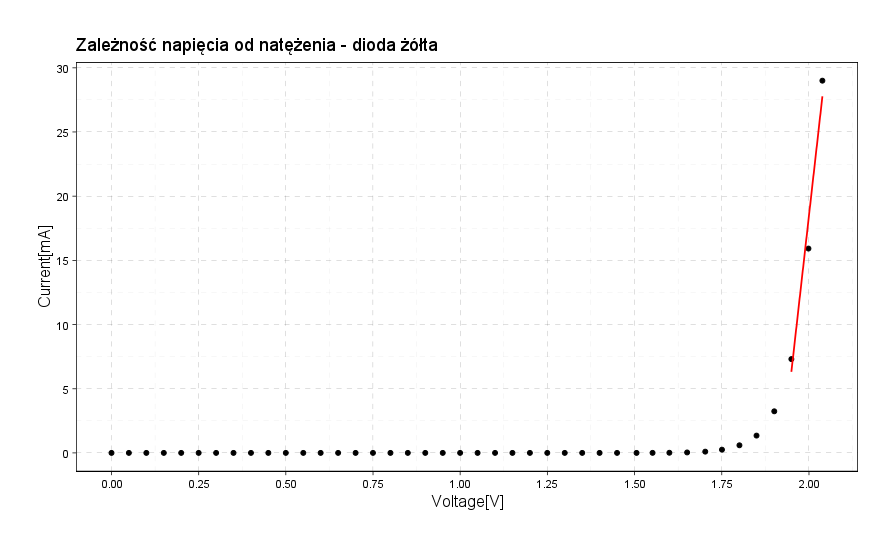
\includegraphics[scale = 0.5]{"Img/Rplot01.png"}\\
    Można zauważyć że na wykresie nie występuję moment wypłaszczenia charakteryzujący moment przemiany fazowej.
    Oznacza to że nie udało się prawidłowo przeprowadzić doświadczenia i niemożliwym jest wyliczenie temperatury krzepnięcia wody.

    \subsection*{Skalowanie termopary}
    \indent Współczynnik termoelektryczny termopary wyznaczono korzystając z regresji liniowej.\\
    \begin{gather*}
        \alpha=0.040545\pm 0.00032[\frac{mV}{^\circ C}]
    \end{gather*}
    Na podstawie współczynnika oraz badanego napięcia
    podczas skalowania termopary możemy wyznaczyć temperaturę badaną w danym momencie i porównać wyniki z
    pomiarami termometru:
    \begin{center}
        \csvreader[tabular = |c|c|c|c|,
            table head = \hline \textbf{T[$^\circ$C]} & \textbf{Napięcie[V]}& \textbf{\boldmath$T_\alpha$[$^\circ$C]}& \textbf{T-\boldmath$T_\alpha$[$^\circ$C]}\\\hline,
            late after line = \\\hline
        ]{Dane/Wyniki1.csv}{}{
            \csvcoli & \csvcolii & \csvcoliii & \csvcoliv
        }
    \end{center}
    {\footnotesize
        \begin{itemize}
            \item[] \textbf{T} - temperatura mierzona termometrem,
            \item[] \boldmath{$T_\alpha$} - temperatura wyliczona na podstawie współczynnika $\alpha$,
        \end{itemize}}

    \indent Można zauważyć że między wartością zmierzoną termometrem a wartością obliczoną
    występuję różnica o wiele wykraczająca od wartości wyliczonego błędu pomiarowego.
    Wynika to prawdopodobnie z błędnego założenia że niepewność pomiarowa regresji liniowej jest równoważna niepewności
    współczynnika termopary. Na niepewność regresji liniowej wpływa również błąd pomiaru temperatury oraz błąd pomiaru napięcia.
    Należałoby więc policzyć niepewność złożoną z regresji liniowej uwzględniając niepewności wartości mierzonych.\\

    \newpage

    \indent Z źródeł zewnętrznych uzyskano inną metodę wyznaczania współczynnika termoelektrycznego termopary:
    \begin{gather*}
        \alpha=\frac{\Delta U}{\Delta T}
    \end{gather*}
    {\footnotesize
        \begin{itemize}
            \item[] $\Delta U$ - średnia mierzonej różnicy potencjałów między zaciskami termopary,
            \item[] $\Delta T$ - średnia temperatury,
        \end{itemize}}
    \noindent Ze wzoru uzyskano wartość współczynnika:
    \begin{gather*}
        \alpha=0.039[\frac{mV}{^\circ C}]
    \end{gather*}
    \noindent Porównując wyniki tak jak powyżej:
    \begin{center}
        \csvreader[tabular = |c|c|c|c|,
            table head = \hline \textbf{T[$^\circ$C]} & \textbf{Napięcie[V]}& \textbf{\boldmath$T_\alpha$[$^\circ$C]}& \textbf{T-\boldmath$T_\alpha$[$^\circ$C]}\\\hline,
            late after line = \\\hline
        ]{Dane/Wyniki2.csv}{}{
            \csvcoli & \csvcolii & \csvcoliii & \csvcoliv
        }
    \end{center}
    Można zauważyć że różnica między wynikami w tym przypadku jest zauważalnie mniejsza.
    \indent Metoda wykorzystująca regresję liniową jest bardzo podatna na błędy wynikające z przeprowadzonej formy skalowania termopary.
    Sposobami na poprawienie wyniku wynikającego z regresji byłoby podgrzewanie wody w garnku wolniej aby mieć większą kontrolę nad temperaturą.
    Jednak ostatecznie należałoby skłonić się ku metodom alternatywnym wyznaczania wartości współcznnika termoelektrycznego.\\
    \indent Wyznaczone współczynniki odpowiadają współczynnikom dla termopary typu T(Miedź-Konstantan) oraz termopary typu K(Chromel-Alumenl) których współczynnik
    termoelektryczny wynosi około 0.040[$\frac{mV}{^\circ C}$].\\\\
    \begin{center}
        \small \textbf{Uwaga} - Dane w tabelach nie zostały zaokrąglane umyślnie w celu łatwiejszej analizy danych.
    \end{center}

\end{document}